\documentclass[12pt]{article}

\usepackage{color, graphicx, float, hyperref}

\begin{document}
\title{Numerically Solving Advection-Diffusion-Reaction Equations}
\author{Carl Denton}
\maketitle

\section{Introduction}

Advection-Diffusion-Reaction (ADR) Equations are partial differential equations (PDEs) of the form
\[\frac{\partial}{\partial t} \varphi + U\nabla \cdot \varphi = D\nabla^2\cdot\phi + R(\varphi)\]
That is, they are characterized by the presence of advection: $U\nabla \cdot \varphi$; diffusion: $D\nabla^2 \cdot \varphi$; and arbitrary reaction: $R(\varphi)$.
They encompass a wide range of phenomena including diffusion (for example of heat or fluid), atmospheric transport, various chemical phenomena, bacterial growth, and more. 
Thus it is desirable to simulate their solutions and we do so here.

\vspace{1pc}

\noindent Code for the following can be found at \url{https://github.com/cfdenton/ac274}

\section{Methods}

\subsection{Numerical Differentiation}

We can compute numerical derivatives by the method of finite differences. By computing Taylor expansions we observe that
\[\varphi'(x) \approx \frac{\varphi(x+dx) - \varphi(x)}{dx} \approx \frac{\varphi(x + dx) - \varphi(x - dx)}{2dx}\]
for some small $dx$, where the first expression is accurate to first order in $dx$ and the second is accurate to second order.
Similarly, we get that
\[\varphi''(x) \approx \frac{\varphi(x+dx) - 2 \varphi(x) + \varphi(x - dx)}{dx^2}.\]

\subsection{Transport Matrix}

Exploiting the fact that the numerical derivatives given above are linear operators in $\varphi$, and assuming that $R(\varphi)$ is also linear in $\varphi$, we can write an update of the ADR equation as
\[\varphi^{n+1} = L\varphi^n\]
where $\varphi^t$ is the state $\varphi$ at some time $t$ and $L$ is a linear operator encompassing the differentiation operations as well as the coefficients of the ADR equation.
If $\varphi^t$ is represented as a vector of $N$ dimensions, then $L$ is a $N\times N$ tridiagonal matrix (in the one-dimensional case). In the two-dimensional case, $L$ has 5 diagonals.
This property can be used to derive useful stability conditions for the simulations.

%{\Huge\color{red} Add more here}

\section{Experiments}

We use python (with the NumPy package) for the numerics, and we use GnuPlot and the VisPy package for visualizing the results. By the above analysis, we can execute the simulation by constructing an initial state and a transport matrix, and obtain subsequent states by iteratively multiplying the transport matrix by the state at any given time.

\subsection{Single Dimension}
\subsubsection{Transport Matrix}
We have the following:
\[\frac{\varphi^{n+1}_j - \varphi^n_j}{dt} = -U\frac{\varphi^n_{j+1} - \varphi^n_{j-1}}{2dx} + D\frac{\varphi^n_{j+1} - 2\varphi^n_j + \varphi^n_{j-1}}{dx^2} + R(\varphi)\]
where we say that $\varphi_{j+1} = \varphi(x + dx)$ and we choose $dx$ and $dt$ to be some sufficiently small numbers. Under this representation, assuming that $R(\varphi^n_j) = R\varphi^n_j$ we get that $L$ is a tridiagonal matrix $\{a, c, b\}$ where 
\[a = dt\left(\frac{D}{dx^2}-\frac{U}{2dx}\right)\]
\[b = dt\left(\frac{D}{dx^2}+\frac{U}{2dx}\right)\]
and 
\[c = 1 - 2dt\frac{D}{dx^2} + R\]
\subsubsection{Diffusion}
We set our initial condition to be a tall gaussian in the middle of the mesh. The results are plotted below at time steps 0, 500, 1000, and 2000 with a grid size of 1000:

\[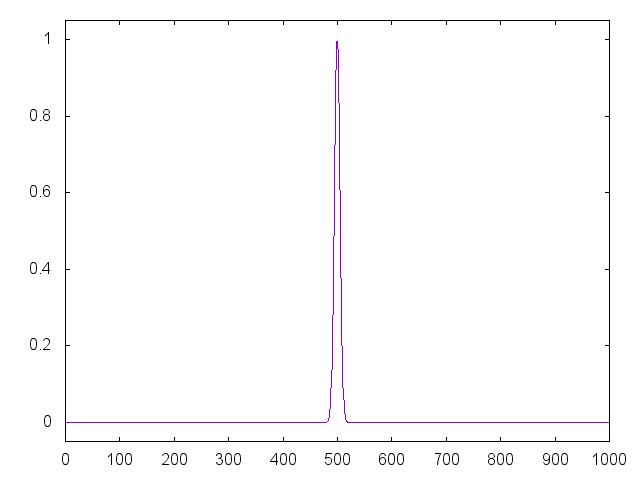
\includegraphics[width=.5\hsize]{adr1d-state-0.png} 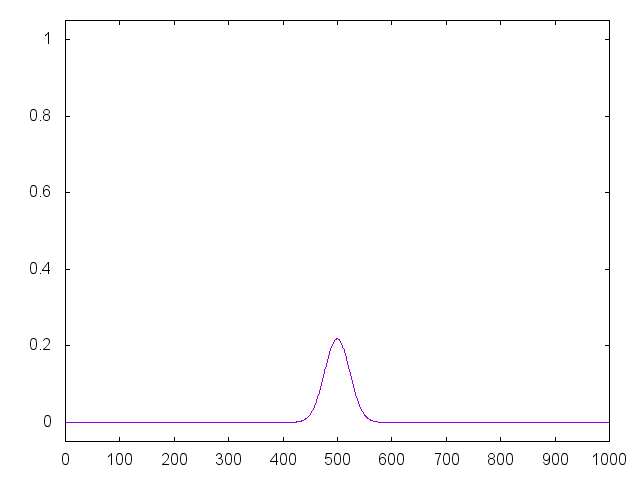
\includegraphics[width=.5\hsize]{adr1d-state-500.png}\] 
\[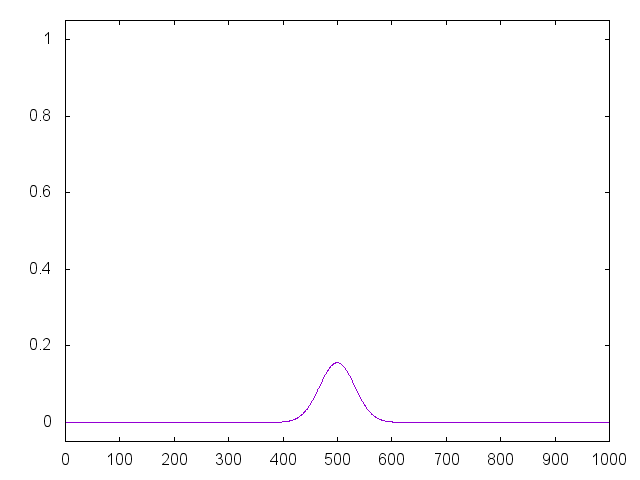
\includegraphics[width=.5\hsize]{adr1d-state-1000.png}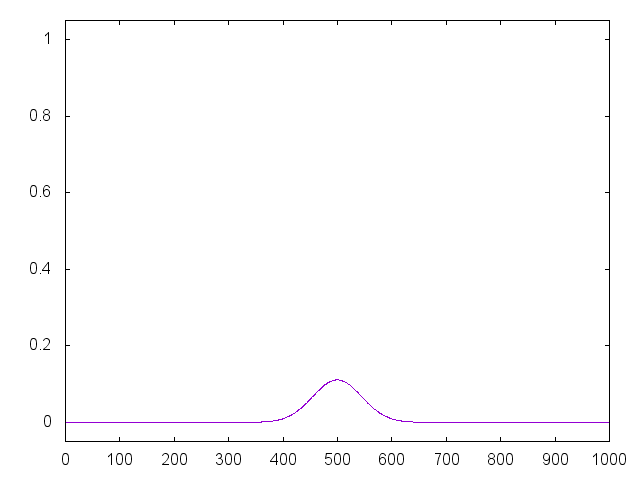
\includegraphics[width=.5\hsize]{adr1d-state-2000.png}\]

\noindent These correspond well with our intuition for a diffusive process--- we will do a more formal validation of the results in section 4.

\subsubsection{Diffusion+Advection}
We can repeat the above experiment while adding advection by adding a nonzero ``$U$" term.
The results are as follows, again at time steps 0, 500, 1000, and 2000:

\[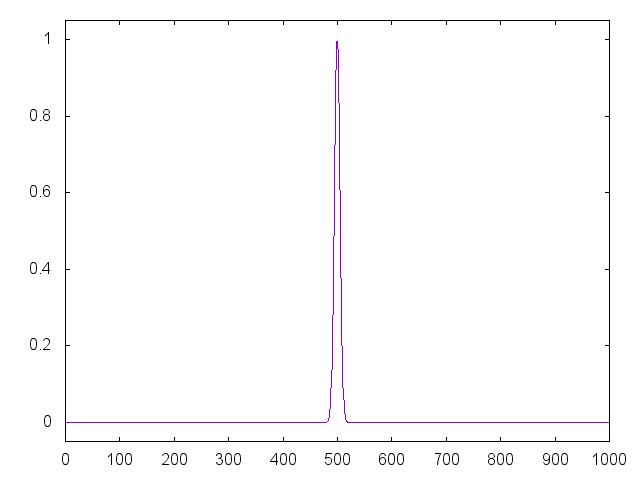
\includegraphics[width=.5\hsize]{adr1d-state-0.png} 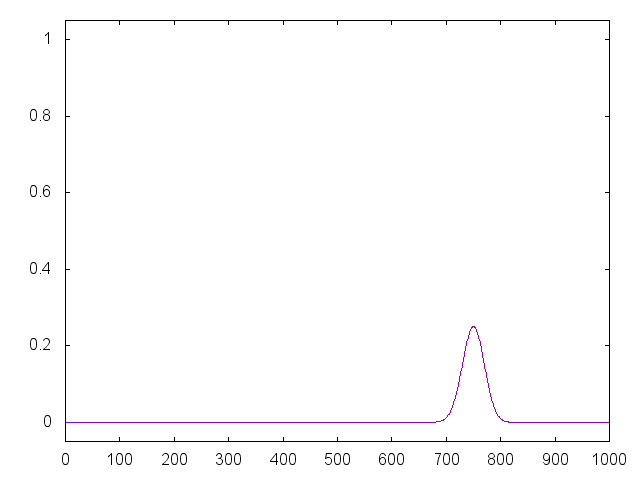
\includegraphics[width=.5\hsize]{adr1d-state-adv500.png}\] 
\[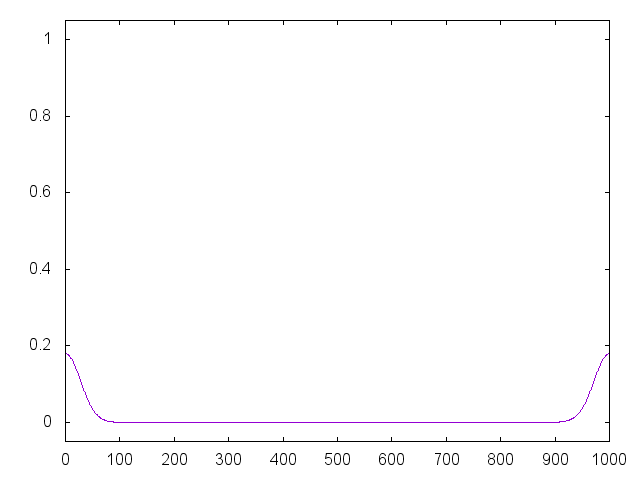
\includegraphics[width=.5\hsize]{adr1d-state-adv1000.png}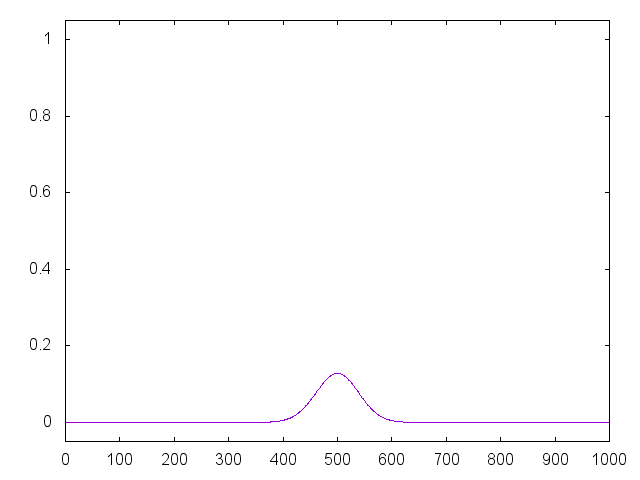
\includegraphics[width=.5\hsize]{adr1d-state-adv2000.png}\]
Note that since we have set periodic boundary conditions, the wave reappears on the left side of the screen after leaving the right side.


\subsubsection{Diffusion+Advection+Reaction}

Finally we add a small amount of positive reaction and obtain the following (at $t = 0, 500, 1000, 2000$):
\[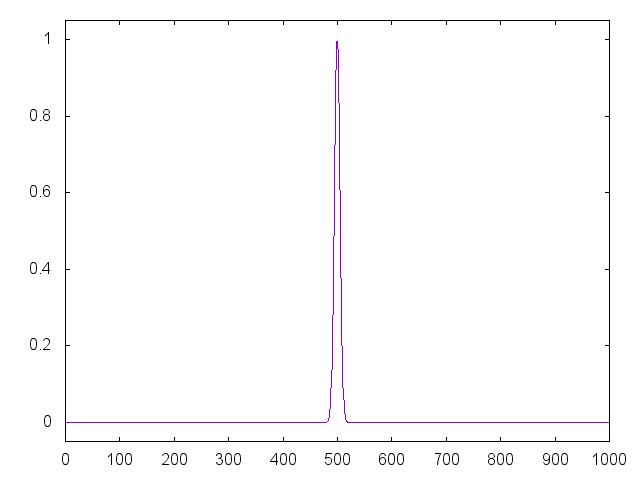
\includegraphics[width=.5\hsize]{adr1d-state-0.png} 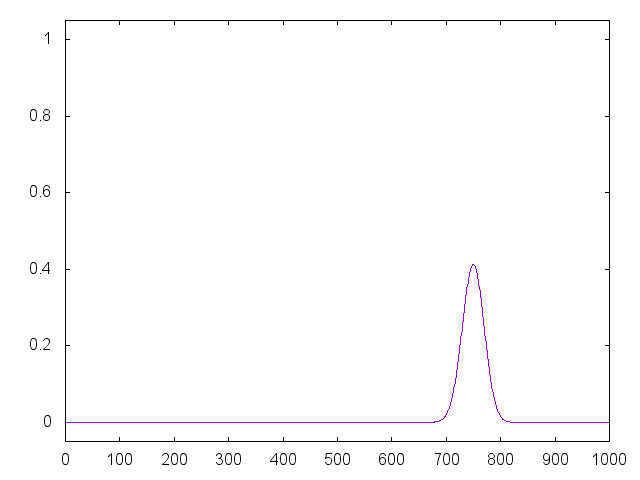
\includegraphics[width=.5\hsize]{adr1d-state-reac500.png}\] 
\[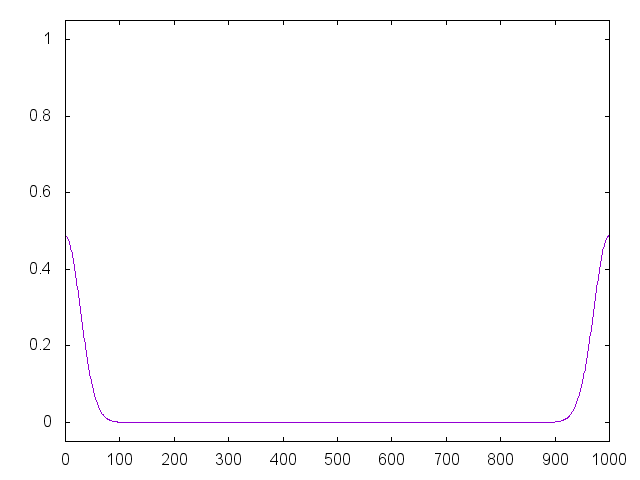
\includegraphics[width=.5\hsize]{adr1d-state-reac1000.png}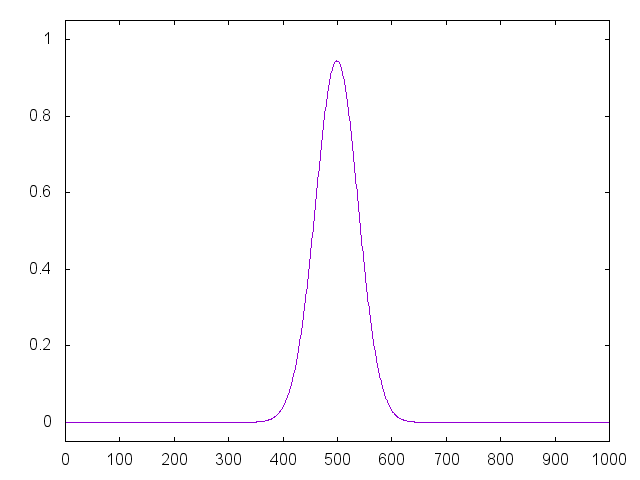
\includegraphics[width=.5\hsize]{adr1d-state-reac2000.png}\]


\subsection{Two Dimensions}

We repeat the experiments in two dimensions:

\subsubsection{Diffusion}
With $t = 0, 500, 1000, 2000$:
\[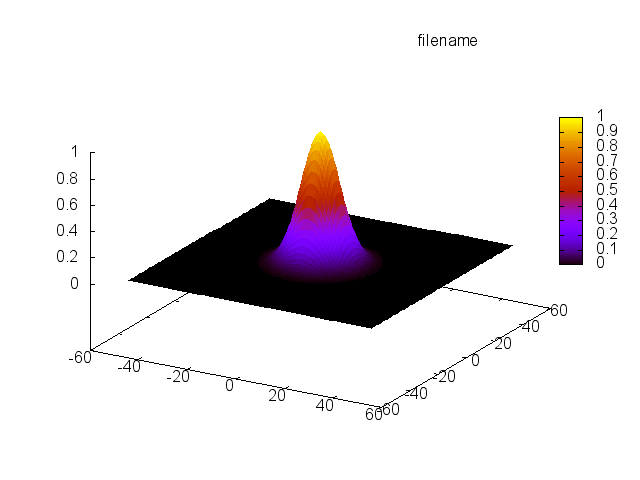
\includegraphics[width=.5\hsize]{adr2d-state-0.png} 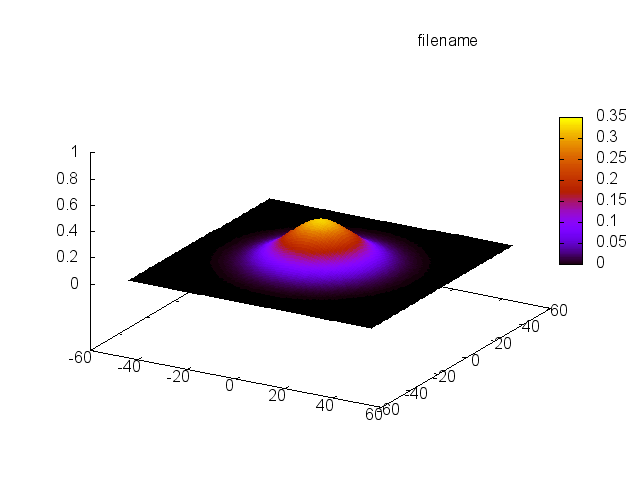
\includegraphics[width=.5\hsize]{adr2d-state-500.png}\] 
\[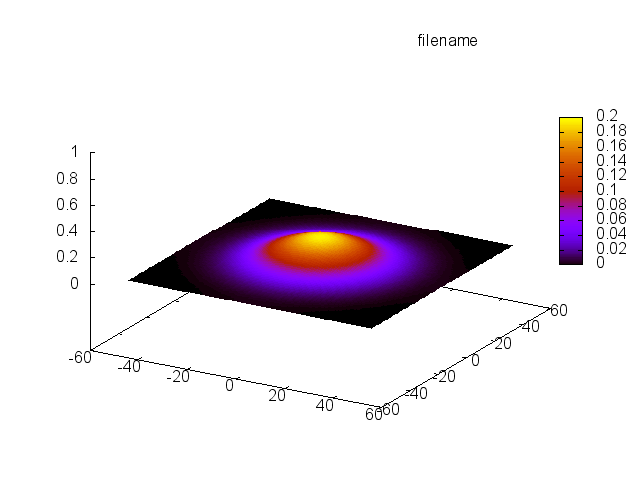
\includegraphics[width=.5\hsize]{adr2d-state-1000.png}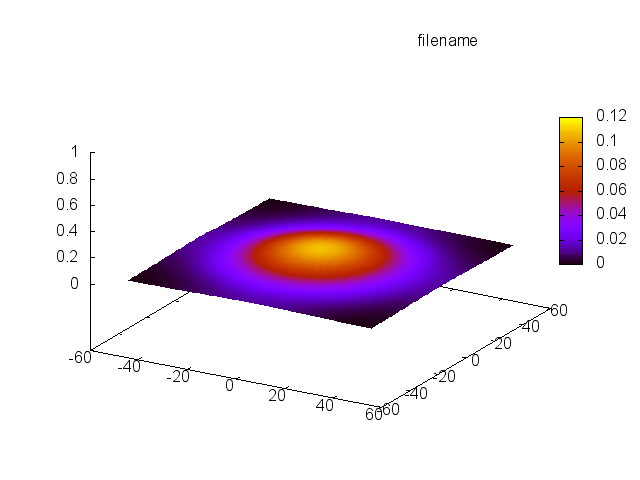
\includegraphics[width=.5\hsize]{adr2d-state-2000.png}\]


\subsubsection{Diffusion+Advection}
With $t = 0, 250, 500, 750$:
\[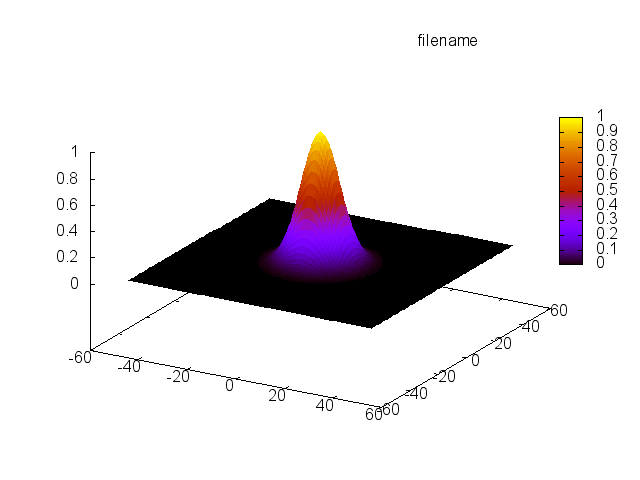
\includegraphics[width=.5\hsize]{adr2d-state-adv0.png} 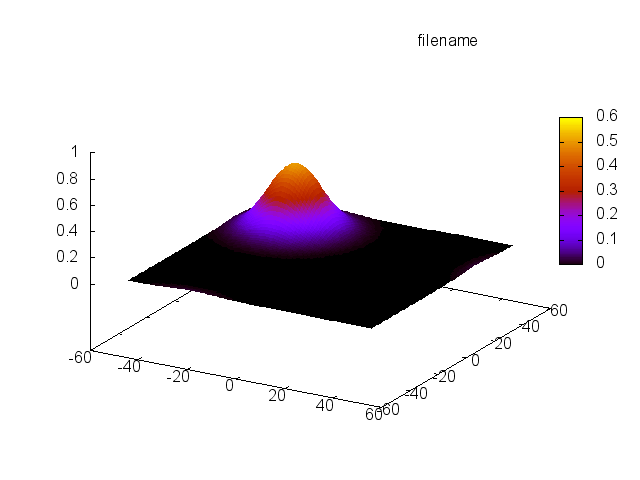
\includegraphics[width=.5\hsize]{adr2d-state-adv250.png}\] 
\[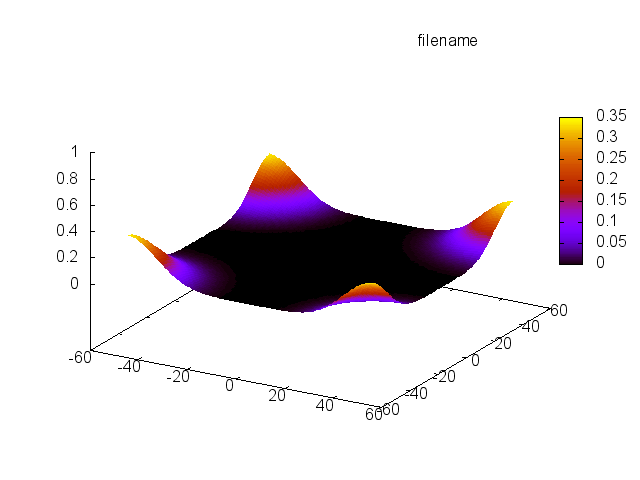
\includegraphics[width=.5\hsize]{adr2d-state-adv500.png}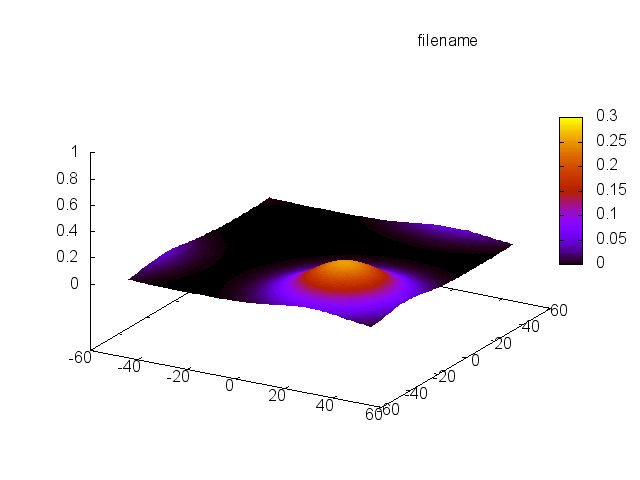
\includegraphics[width=.5\hsize]{adr2d-state-adv750.png}\]

\subsubsection{Diffusion+Advection+Reaction}
With $t = 0, 250, 500, 750$:
\[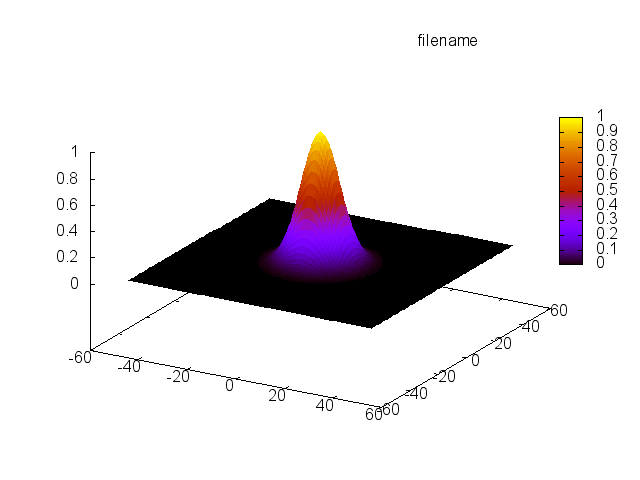
\includegraphics[width=.5\hsize]{adr2d-state-reac0.png} 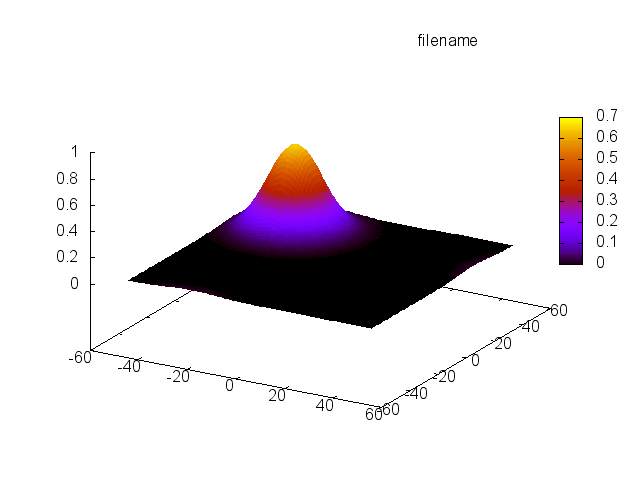
\includegraphics[width=.5\hsize]{adr2d-state-reac250.png}\] 
\[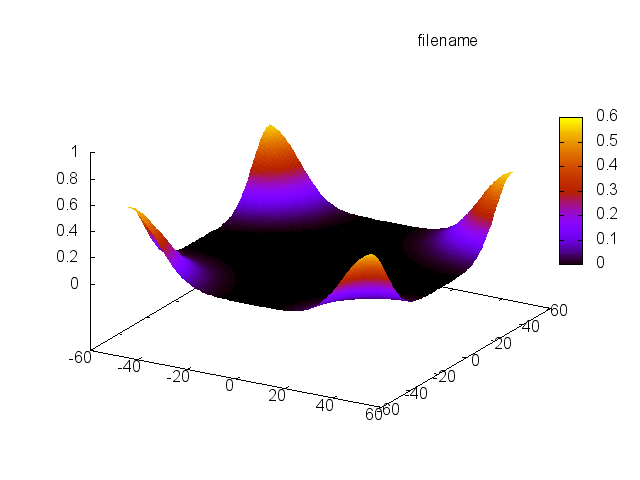
\includegraphics[width=.5\hsize]{adr2d-state-reac500.png}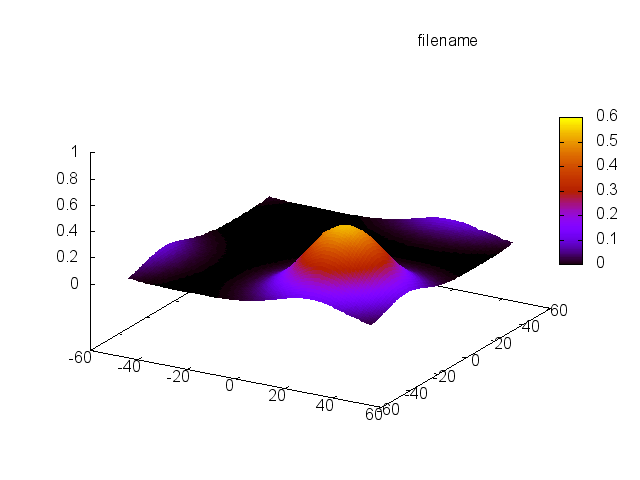
\includegraphics[width=.5\hsize]{adr2d-state-reac750.png}\]

\subsubsection{Nonlinear Chemistry}
We also implement a few types of non-linear chemistry. This can be accomplished by adding the necessary term to the state after the transport matrix has been applied. First we model logistic growth as $R(\varphi) = R\varphi(1-\varphi)$:

\[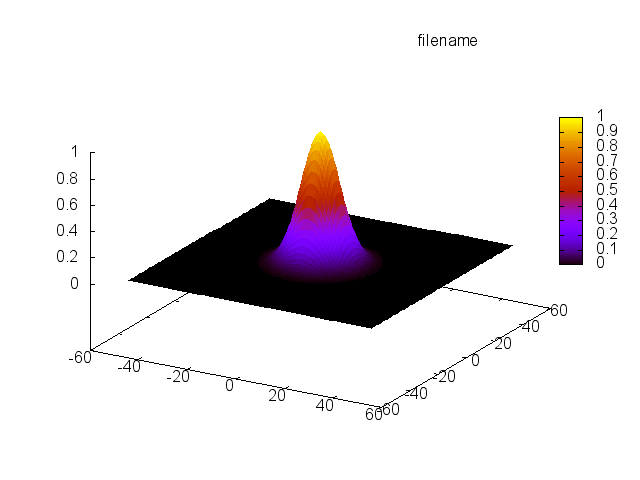
\includegraphics[width=.5\hsize]{adr2d-state-log0.png} 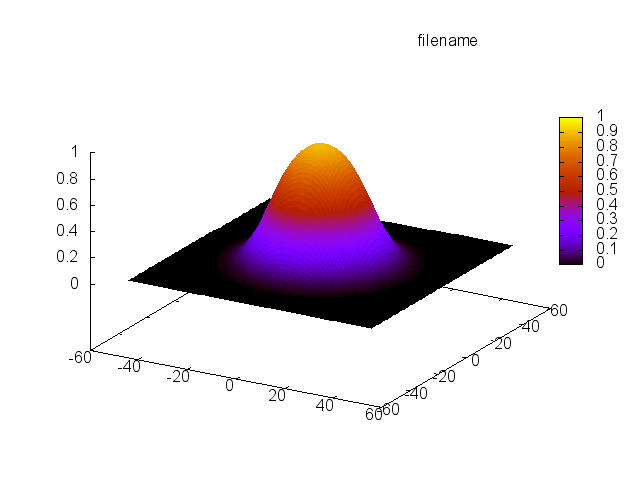
\includegraphics[width=.5\hsize]{adr2d-state-log250.png}\] 
\[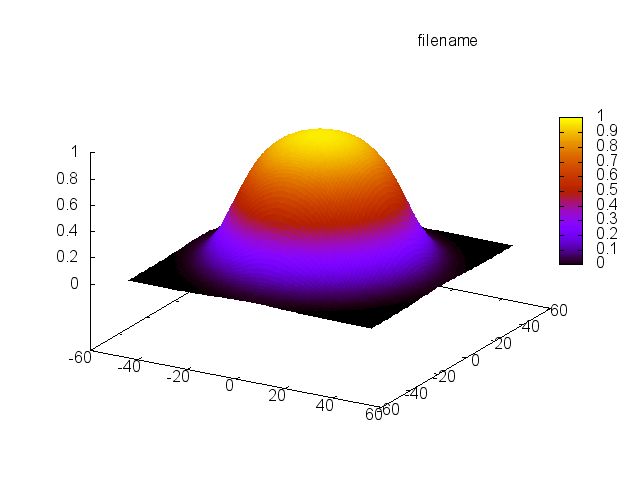
\includegraphics[width=.5\hsize]{adr2d-state-log500.png}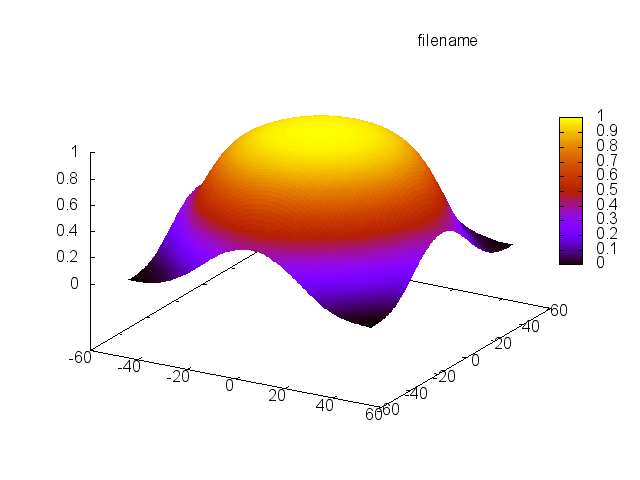
\includegraphics[width=.5\hsize]{adr2d-state-log750.png}\]

As expected, the concentration plateaus at $\varphi = 1$.
Following the demonstration in class, we also model chemistry of the form $R(\varphi) = a(x, y)\varphi - b \varphi^2$, where $a(x, y)$ is a randomly varying function of the position. The initial configuration is also a small random variation, and as a result we obtain a highly random final distribution:
\[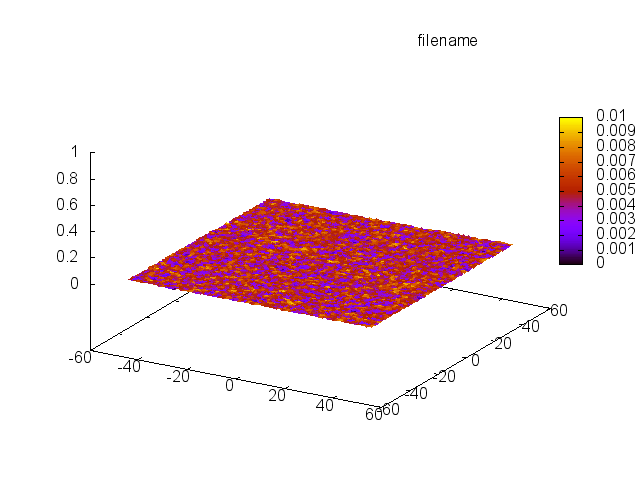
\includegraphics[width=.5\hsize]{adr2d-state-rand0.png} 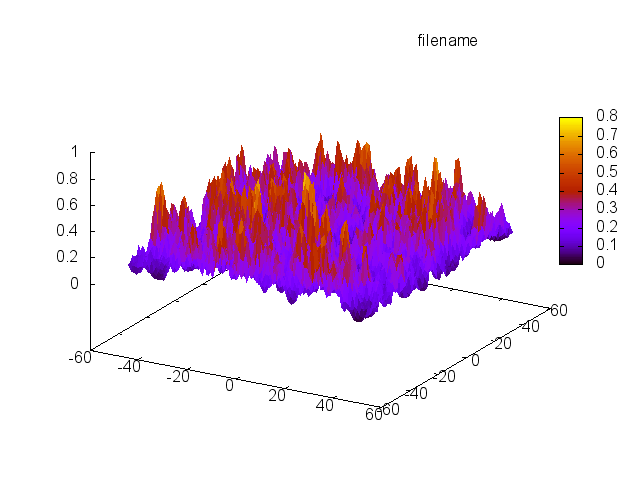
\includegraphics[width=.5\hsize]{adr2d-state-rand250.png}\] 
\[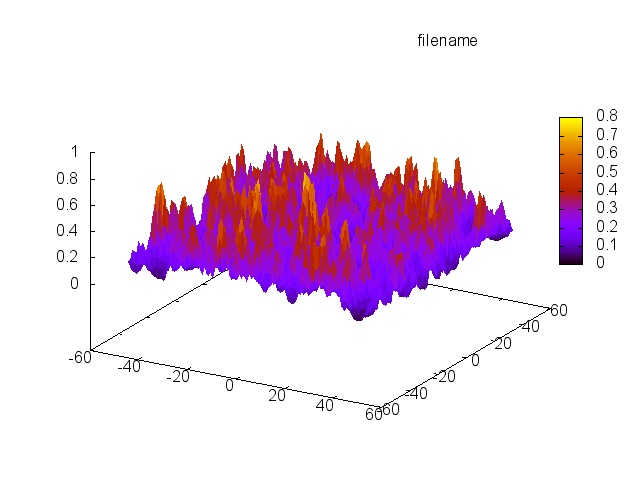
\includegraphics[width=.5\hsize]{adr2d-state-rand500.png}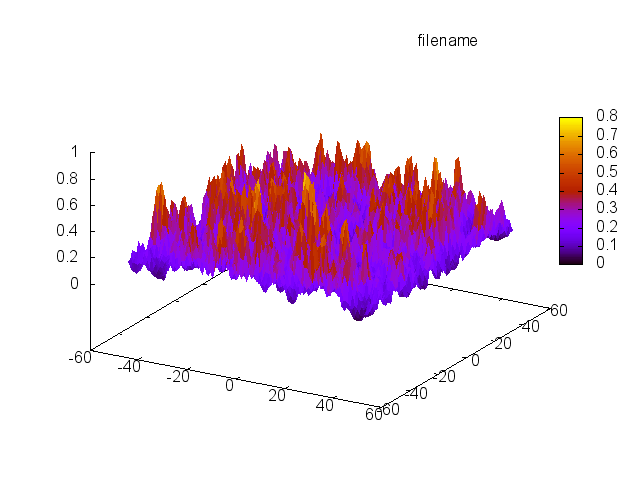
\includegraphics[width=.5\hsize]{adr2d-state-rand750.png}\]
We also manage to replicate the types of striations found in the work from class:
\[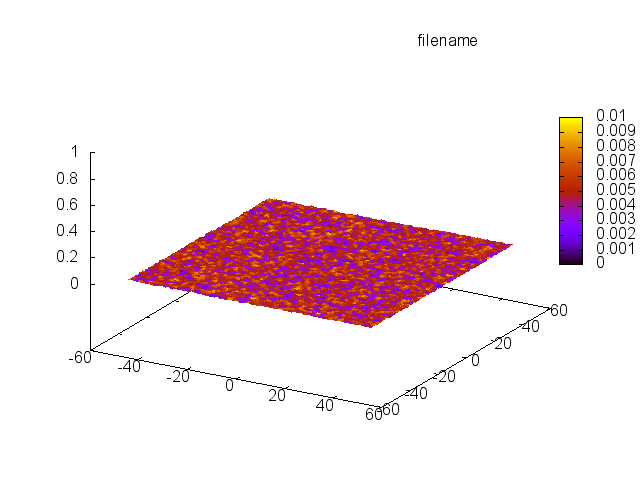
\includegraphics[width=.5\hsize]{adr2d-state-rand-adv0.png} 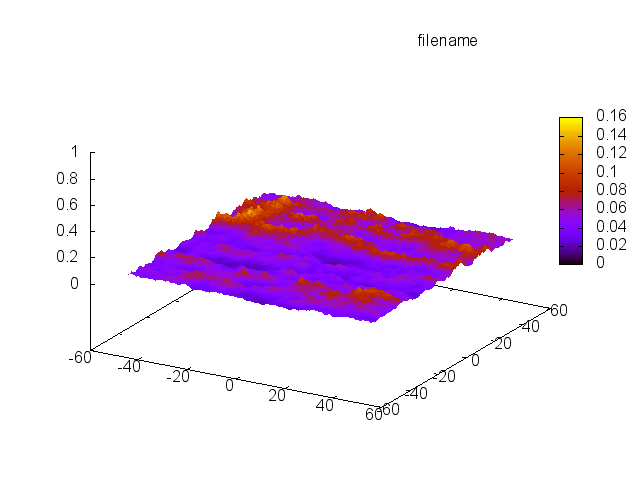
\includegraphics[width=.5\hsize]{adr2d-state-rand-adv250.png}\] 
\[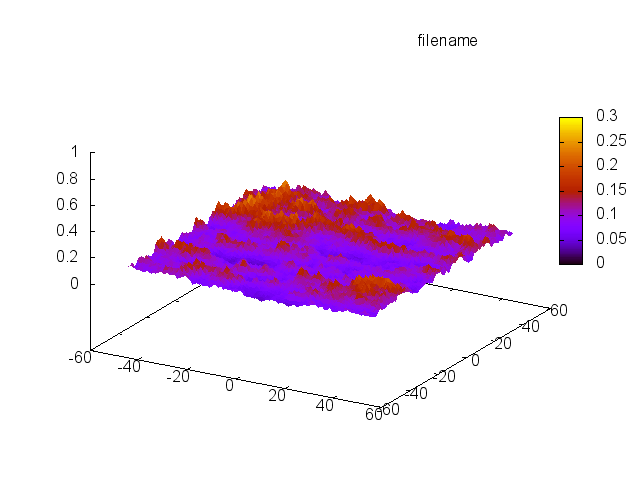
\includegraphics[width=.5\hsize]{adr2d-state-rand-adv500.png}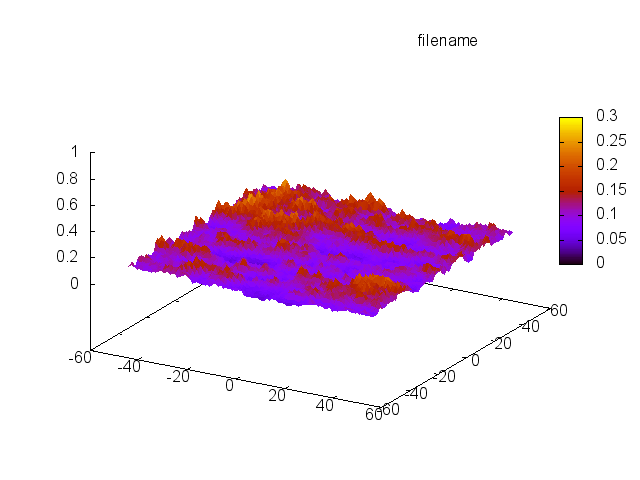
\includegraphics[width=.5\hsize]{adr2d-state-rand-adv750.png}\]


\section{Analysis}

\subsection{Comparison with Analytic Solutions}

We plot the mass, average position, variance, and entropy of the system over time to validate our simulation. In the one dimensional case, we get:
\begin{figure}[H]
\caption{Mass and Average Position}
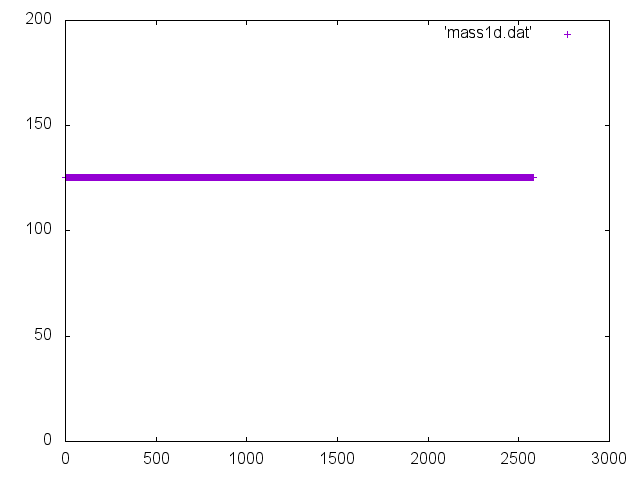
\includegraphics[width = .5\hsize]{mass1d.png}
\hfill
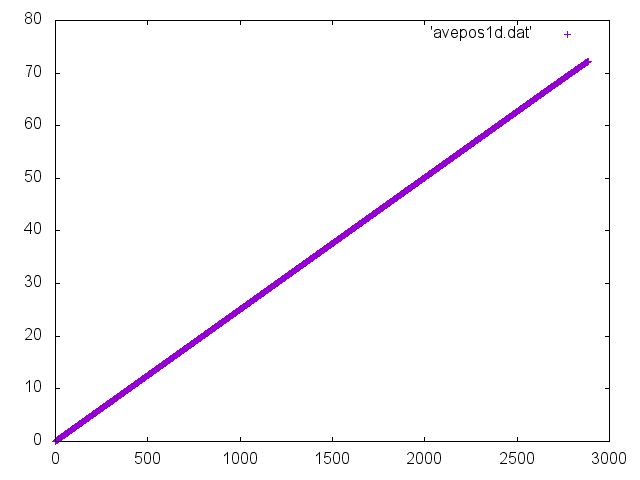
\includegraphics[width = .5\hsize]{avepos1d.png}\end{figure}

\begin{figure}[H]
\caption{Variance and Entropy }
\[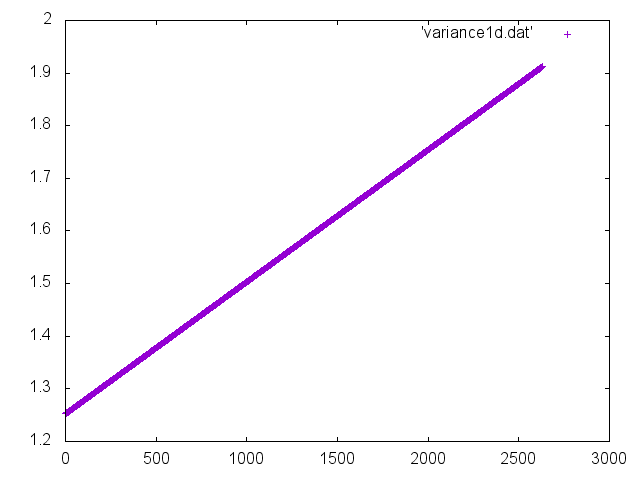
\includegraphics[width = .5\hsize]{variance1d.png}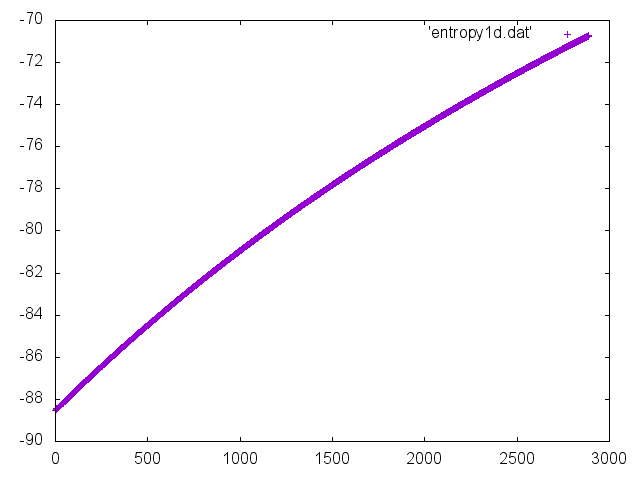
\includegraphics[width = .5\hsize]{entropy1d.png}\]
\end{figure}

These correspond well with the predictions of analytic solutions. Analogues hold in the two dimensional case.





\end{document}
